\chapter{Diseño del datamart analítico}
\label{chap:diseno_datamart}

\lettrine{E}{l} diseño del Datamart constituye el núcleo lógico de este proyecto. Se ha optado por un modelo dimensional en estrella (Star Schema) basado en la metodología de Ralph Kimball, pero introduciendo optimizaciones específicas para tratar variables demográficas de alta cardinalidad e historificación de expedientes.

\section{Modelo dimensional en estrella}

A diferencia de las bases de datos transaccionales, que están altamente normalizadas, el esquema del Data Warehouse se ha desnormalizado en dos tipos de tablas: \textbf{tablas de hechos} (que almacenan métricas y claves foráneas) y \textbf{tablas de dimensiones} (que contienen descriptores textuales para filtrar y agrupar).

En nuestro diseño final se han establecido dos tablas de hechos de diferente granularidad para responder a distintas necesidades analíticas, rodeadas por un total de siete dimensiones. La figura \ref{fig:datamart_erd} muestra el esquema completo del Datamart, con todas las tablas del esquema \textit{dwh}, sus columnas, claves primarias, claves foráneas y las relaciones entre ellas.

\begin{figure}[htbp]
    \centering
    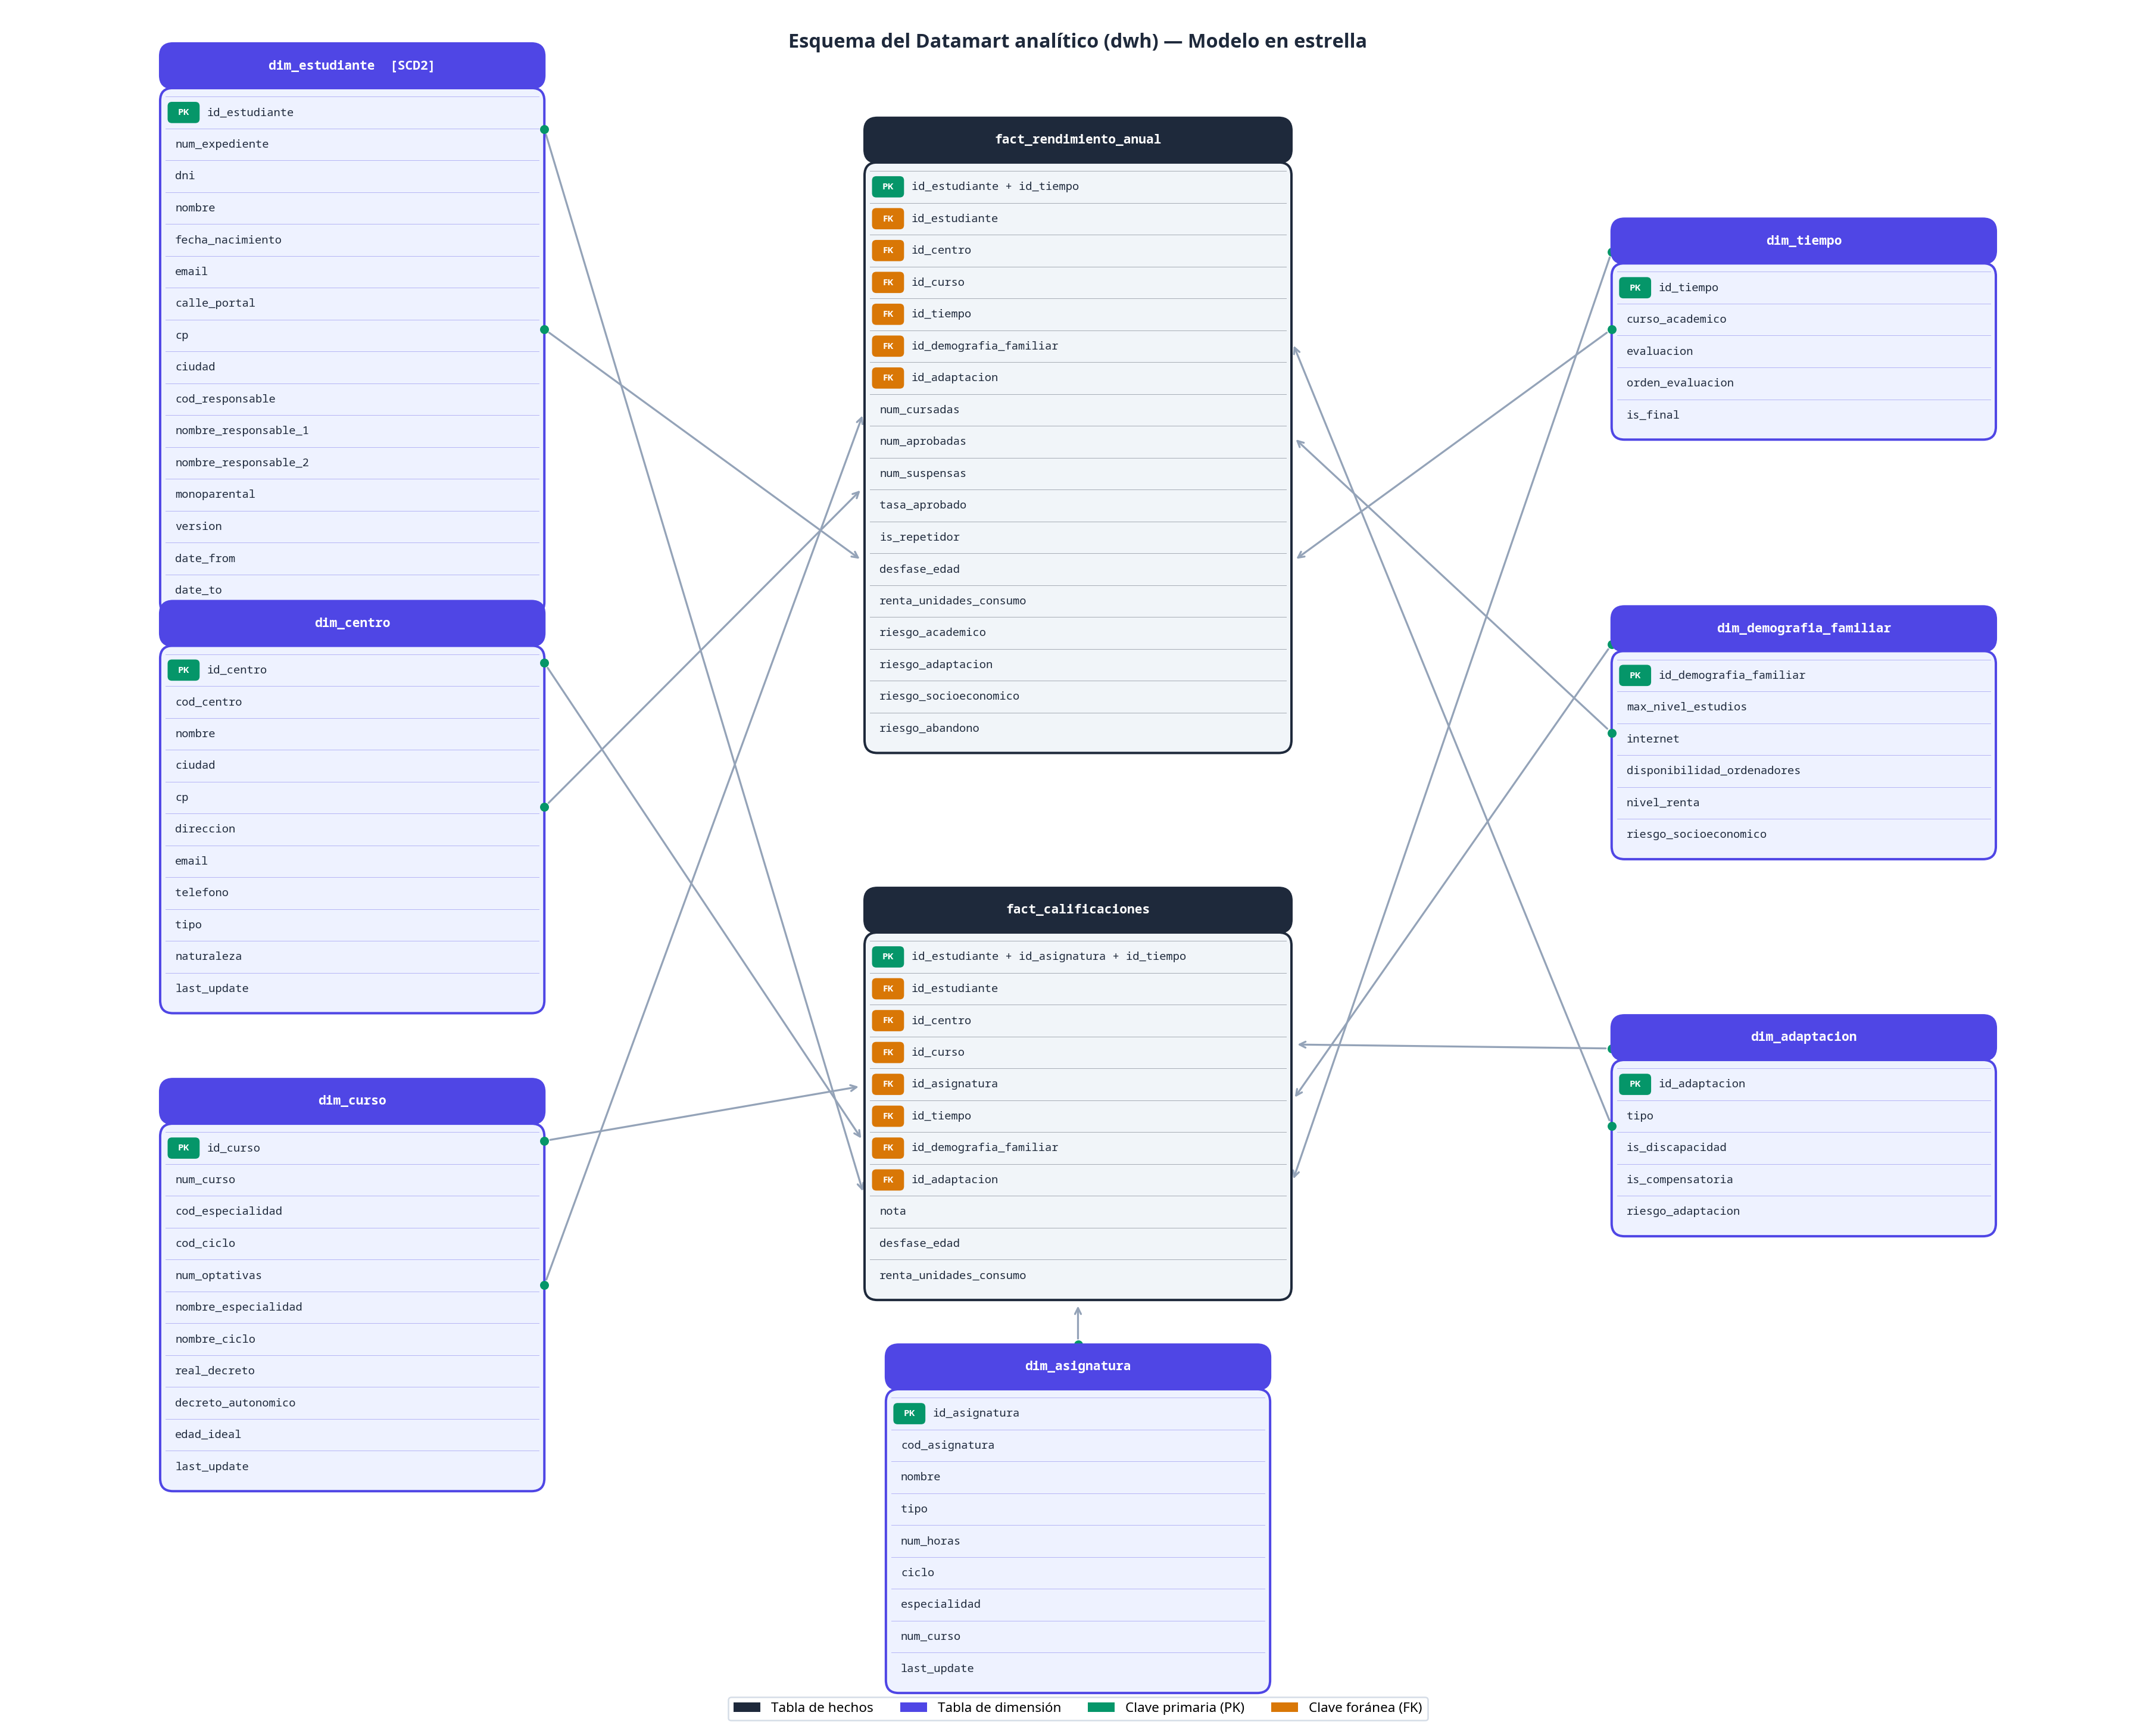
\includegraphics[width=1.2\textwidth]{imaxes/fig_datamart_erd}
    \caption{Esquema del Datamart analítico (\textit{dwh}) en modelo estrella.}
    \label{fig:datamart_erd}
\end{figure}

\subsection{Tablas de dimensiones en detalle}

Las dimensiones contextualizan los datos numéricos. Para este proyecto se han diseñado las siguientes:

\begin{itemize}
    \item \textbf{\textit{dim\_estudiante} (SCD Tipo 2):} Contiene los datos personales del alumno y su responsable legal. Para reflejar la inestabilidad habitacional o cambios de tutela (muy comunes en entornos vulnerables), se implementó una \textit{dimensión de variación lenta de tipo 2 (SCD2)}. Esto significa que ante un cambio de tutor o domicilio, no se sobrescribe la fila, sino que se caduca (marcando una fecha de fin) y se crea una nueva, preservando el contexto histórico de las notas de años anteriores.
    \item \textbf{\textit{dim\_centro}:} Almacena la información institucional y geográfica de los colegios e institutos.
    \item \textbf{\textit{dim\_curso}:} Consolida la estructura académica (Ciclo, Especialidad y Curso).
    \item \textbf{\textit{dim\_asignatura}:} Catálogo de materias independientes del currículo, con su carga horaria.
    \item \textbf{\textit{dim\_tiempo}:} Dimensión temporal que almacena el año académico y el periodo de evaluación.
    \item \textbf{\textit{dim\_demografia\_familiar}:} Utiliza un modelo demográfico híbrido para reducir la cardinalidad. En lugar de almacenar ingresos exactos, clasifica a las familias por su nivel de renta en tramos, conectividad a internet y disponibilidad de ordenadores.
    \item \textbf{\textit{dim\_adaptacion}:} Registra si el alumno cuenta con adaptaciones curriculares, categorizándolas por discapacidad médica o compensación sociopedagógica.
\end{itemize}

\subsection{Tablas de hechos}

El modelo implementa dos niveles de análisis a través de dos tablas de hechos:

\begin{itemize}
    \item \textbf{\textit{fact\_calificaciones} (Granularidad Atómica):} Representa el nivel más detallado. Cada fila es la nota exacta de un estudiante en una asignatura durante una evaluación concreta. Es útil para rastrear el progreso pormenorizado a lo largo del curso.
    \item \textbf{\textit{fact\_rendimiento\_anual} (Granularidad Agregada):} Cada fila representa el resumen académico total de un alumno en un curso completo. Consolida el número de asignaturas matriculadas, aprobadas, la tasa de éxito, las asignaturas arrastradas de años anteriores y si el alumno ha repetido. Es en esta tabla donde se calculan de manera definitiva los KPIs críticos y el índice de Riesgo de Abandono Escolar Temprano.
\end{itemize}

\section{Reglas de negocio y cálculo de riesgos}

Para que el Dashboard ofrezca métricas accionables a nivel autonómico, se han parametrizado dos indicadores de riesgo fundamentales mediante sistemas de puntuación acumulativa, integrados en la lógica del Datamart.

\subsection{Riesgo socioeconómico}
Este riesgo evalúa el contexto familiar de exclusión y brecha digital. Los puntos se calculan sumando los siguientes factores:

\begin{itemize}
    \item \textbf{Estudios de los Progenitores (Estándar PARED):} Se ha adoptado el enfoque de la OCDE en sus informes PISA, donde el riesgo correlaciona con el mayor nivel educativo alcanzado por cualquiera de los padres \cite{OECD_PISA}. Puntuaciones aplicadas a cada progenitor: Sin estudios de primaria (5 pts), Primaria (3 pts), Secundaria o superior (1 pt).
    \item \textbf{Renta por Unidades de Consumo (Escala OCDE Modificada):} Para determinar el riesgo económico no se divide la renta de forma puramente lineal (per cápita). Siguiendo la metodología AROPE de Eurostat y las directrices del INE \cite{INE_ECV, EAPN_Pobreza}, la escala teórica estipula que el primer adulto computa como $1$ unidad de consumo, los integrantes mayores de 14 años como $0,5$ unidades y los menores de 14 años como $0,3$. No obstante, debido a que el sistema transaccional de origen no recopila la edad exacta del resto de convivientes (hermanos o familiares), ha sido necesario aplicar una adaptación metodológica en la ETL. Se asigna un peso de $1$ al primer integrante y de $0,5$ al resto, independientemente de su edad. En base a los ingresos anuales equivalentes obtenidos tras la ponderación, se establecen los siguientes niveles de renta en la capa de transformación:
    \begin{itemize}
        \item \textbf{Muy baja (pobreza severa):} Ingresos por unidad de consumo inferiores a 7.000 €/año. Supone una alta penalización (15 pts).
        \item \textbf{Baja (umbral de pobreza):} Ingresos por unidad de consumo entre 7.000 € y 11.000 €/año. Supone una penalización moderada (7 pts).
        \item \textbf{Media/alta:} Ingresos por unidad de consumo superiores a 11.000 €/año. Ambas categorías se han unificado ya que no suponen un factor de riesgo económico y, por tanto, no suman puntos (0 pts).
    \end{itemize}
    \item \textbf{Brecha Digital (Conectividad):} Sin acceso a Internet en el hogar (3 pts).
    \item \textbf{Brecha Digital (Hardware):} 0 ordenadores (5 pts), menos de 1 ordenador por hijo (2 pts).
\end{itemize}
\textit{Nota:} Si la suma del riesgo socioeconómico supera los 16 puntos, la familia se considera en situación de alta vulnerabilidad.

\subsection{Riesgo de abandono del alumno}
Combina factores académicos, de apoyo y de arrastre socioeconómico para emitir una alerta crítica global:

\begin{itemize}
    \item \textbf{Carga del riesgo socioeconómico:} Si en el apartado "riesgo socioeconómico" obtuvo de 16 a 21 puntos (5 pts) en el riesgo de abandono, si son más de 21 (10 pts) .
    \item \textbf{Penalización académica temprana (1.º o 2.º de primaria):} Los fracasos en ciclos iniciales marcan un déficit crónico, esto se penaliza calculando curso a curso durante todo el historial académico del alumno. Suspenso en evaluación regular (10 pts), asignatura suspensa a final de curso (20 pts), repetición del curso (40 pts).
    \item \textbf{Penalización académica general (resto de cursos):} Suspenso en evaluación regular (1 pt), asignatura suspensa a final de curso (5 pts), repetición (10 pts).
    \item \textbf{Necesidades de apoyo y adaptación:} Adaptación por motivos de discapacidad (10 pts). Adaptación por otros motivos o compensatoria (5 pts).
\end{itemize}

Estos valores numéricos quedan consolidados en \textit{fact\_rendimiento\_anual}, lo que permite al Backend (FastAPI) entregar al Dashboard de forma instantánea el listado de centros con mayor concentración de alumnado en riesgo inminente de abandono.
